\section{问题二：油价冲击对中国经济的传导}

\subsection{变量特定的局部投影}

人民币原油成本构造为

\begin{equation}
  C_t^{oil}=P_t^{Brent,USD}FX_t^{CNY/USD},\qquad
  c_t=100\Delta\ln C_t^{oil}.
  \label{eq:oilcost}
\end{equation}

结构冲击的来源不同，其宏观含义也不同\cite{tang2010,cross2017,chen2020}。本文分别输入
不利供给、全球需求和石油特定风险冲击；未分解$OilShock$只作约化形式稳健性。局部投影不对整条
脉冲路径施加强递推限制\cite{jorda2005}，但被解释变量必须与程序定义一致。对PPI、CPI、IAV和
人民币原油成本，估计未来水平响应

\begin{equation}
  y_{t+h}=\alpha_h+\theta_hs_t+\rho_hy_{t-1}+\eta_hs_{t-1}
  +\Gamma_h^{\mathsf T}Z_{t-1}+u_{t+h};
  \label{eq:lp-level}
\end{equation}

对汇率则估计相对冲击前基期的累计变化

\begin{equation}
  100(\ln FX_{t+h}-\ln FX_{t-1})
  =\alpha_h+\theta_hs_t+\rho_h\Delta\ln FX_{t-1}
  +\eta_hs_{t-1}+\Gamma_h^{\mathsf T}Z_{t-1}+u_{t+h}.
  \label{eq:lp-fx}
\end{equation}

$Z_{t-1}$包含美元、GPR、月份虚拟变量和疫情阶段。PPI、CPI、成本和汇率估计$h=0,\ldots,12$；
IAV因1至2月结构性缺失，只估计$h\in\{0,3,6,12\}$。使用同源移动块bootstrap和最大$t$统计量
构造95\%联合置信带。对完整月度路径定义响应曲线面积

\begin{equation}
  A_y(H)=\sum_{h=0}^{H}\widehat\theta_{y,h},
  \label{eq:response-area}
\end{equation}

单位为“百分点月”，只描述离散响应曲线的面积，不称为累计经济损失。IAV的四个稀疏期限不求和。

\begin{figure}[htbp]
  \centering
  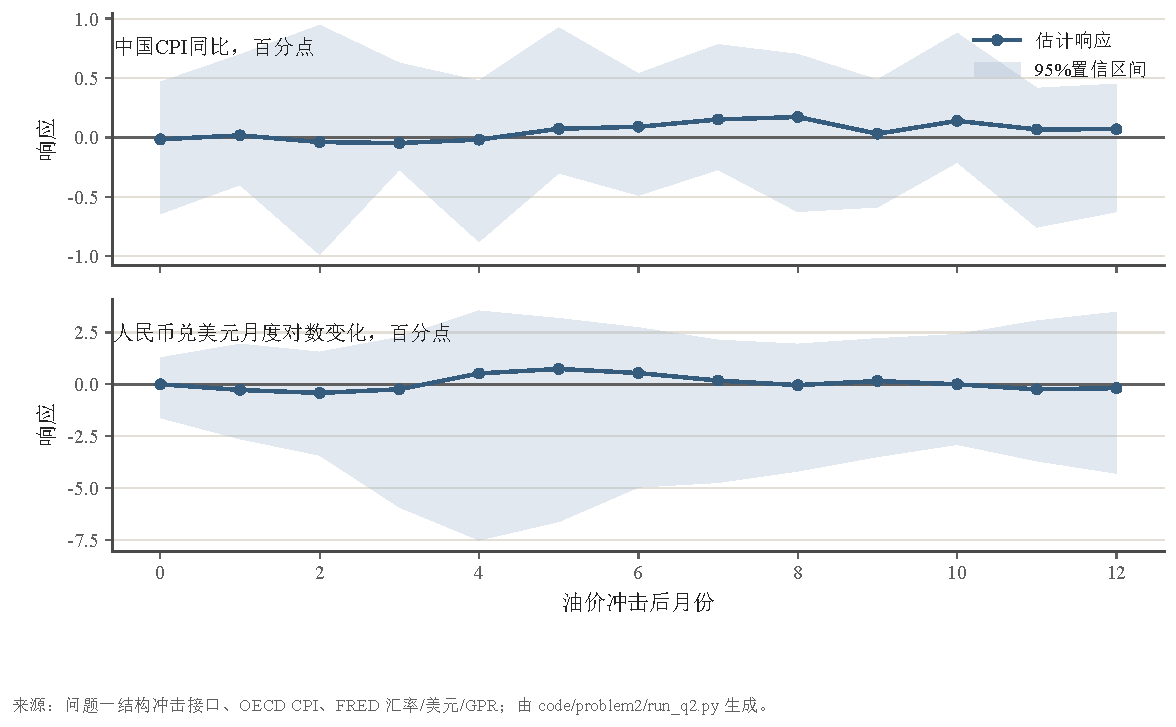
\includegraphics[width=0.91\textwidth]{../figures/q2_irf.pdf}
  \caption{油价特定风险冲击下中国主要变量的局部投影响应}
  \label{fig:q2-irf}
\end{figure}

\subsection{油价特定风险冲击结果}

\begin{table}[htbp]
  \centering
  \small
  \caption{油价特定风险冲击的传导指标}
  \label{tab:q2-metrics}
  \begin{tabularx}{0.98\textwidth}{Xccccc}
    \toprule
    结果变量 & 极值 & 月份 & 极值联合95\%区间 & $A(0,6)$ & $A(0,12)$ \\
    \midrule
    人民币原油成本 & 8.832 & 0 & $[6.888,10.776]$ & 7.440 & 4.939 \\
    PPI同比 & 0.762 & 10 & $[-0.159,1.684]$ & 3.655 & 7.401 \\
    CPI同比 & 0.247 & 7 & $[-0.096,0.589]$ & 0.877 & 2.155 \\
    IAV同比 & $-0.427$ & 12 & $[-0.966,0.111]$ & -- & -- \\
    人民币汇率 & 0.771 & 12 & $[-0.488,2.030]$ & 1.612 & 5.846 \\
    \bottomrule
  \end{tabularx}
\end{table}

成本入口当月响应最清晰；PPI和CPI点估计滞后上行，IAV在12个月出现负向点估计。但除成本入口外，
极值的联合区间均跨零，故不能将点估计写成稳健总体增长损失。季度GDP在加入所需滞后后没有足够
有效观测，低频验证状态为“结论不充分”，也不再报告旧版小样本回归值。

不同结构冲击的响应方向并不相同：全球需求扩张可同时推高油价和产出，不利供给或石油特定风险
更符合成本推动机制。这解释了为何“油价上涨”不能直接等同于“经济受损”。ARDL、疫情剔除、
冲击正负拆分和替代排序只作为稳健性探针；它们未把工业活动和GDP证据提升为联合显著。

\subsection{问题二小结}

模型支持“进口成本快速响应、PPI和CPI滞后上行、工业活动可能承压”的传导顺序，但总体增长损失
仍为结论不充分。后续政策评价必须同时报告物价、工业活动、响应期限和区间，不能只比较单一价格
传导系数。
